%!TEX root=qsic2014.tex
% mainfile: qsic2014.tex

% Jeshua Kracht and Jacob Petrovic

\documentclass[conference]{IEEEtran}
%\makeindex
\usepackage{cite}
\usepackage[hidelinks]{hyperref}
\usepackage[cmex10]{amsmath}
\usepackage{url}
\usepackage{mathtools}
\usepackage[pdftex]{graphicx}
\usepackage{caption}
\usepackage{color}
\usepackage{xspace}
\usepackage{booktabs}

\newcommand{\squishlist}{
 \begin{list}{$\bullet$}
  { \setlength{\itemsep}{0pt}
     \setlength{\parsep}{3pt}
     \setlength{\topsep}{3pt}
     \setlength{\partopsep}{0pt}
     \setlength{\leftmargin}{1.5em}
     \setlength{\labelwidth}{1em}
     \setlength{\labelsep}{0.5em} } }

\newcommand{\squishlisttwo}{
 \begin{list}{$\bullet$}
  { \setlength{\itemsep}{0pt}
     \setlength{\parsep}{0pt}
    \setlength{\topsep}{0pt}
    \setlength{\partopsep}{0pt}
    \setlength{\leftmargin}{2em}
    \setlength{\labelwidth}{1.5em}
    \setlength{\labelsep}{0.5em} } }

\newcommand{\squishend}{
  \end{list}  }


% Comment out one of these two definitions to show/hide comments in the paper
\newcommand{\todo}[1]{\relax}
%\newcommand{\todo}[1]{{\color{red}\bfseries [[#1]]}}

%% Macros for tool names
\def\evo{\textsc{EvoSuite}\xspace}
\def\codepro{CodePro\xspace}
\def\jacoco{Jacoco\xspace}
\def\randoop{Randoop\xspace}
\def\jcrasher{JCrasher\xspace}
\def\palus{Palus\xspace}
\def\testera{TestEra\xspace}

%% Macros for subject programs
\def\netweaver{Netweaver\xspace}
\def\inspirento{Inspirento\xspace}
\def\jsecurity{Jsecurity\xspace}
\def\saxpath{Saxpath\xspace}
\def\jni{Jni-inchi\xspace}
\def\xisemele{Xisemele\xspace}
\def\diebierse{Diebierse\xspace}
\def\lagoon{Lagoon\xspace}
\def\lavalamp{Lavalamp\xspace}
\def\jnfe{Jnfe\xspace}

%% Reduce arraystretch in tables if we need to save space
\renewcommand{\arraystretch}{1.025}

\begin{document}
\title{Empirically Evaluating the Quality of Automatically Generated and Manually Written Test Suites}
% \subtitle{[Extended Abstract]}

\author{\IEEEauthorblockN{Jeshua S. Kracht}
\IEEEauthorblockA{Department of Computer Science\\
University of Colorado, Colorado Springs\\
Email: jkracht@uccs.edu}
\and
\IEEEauthorblockN{Jacob Z. Petrovic}
\IEEEauthorblockA{Department of Computer Science\\
University of Colorado, Colorado Springs\\
Email: jpetrovi@uccs.edu}
\and
\IEEEauthorblockN{Kristen R. Walcott-Justice}
\IEEEauthorblockA{Department of Computer Science\\
University of Colorado, Colorado Springs\\
Email: kjustice@uccs.edu}}

\maketitle
\begin{abstract}
\todo{Define the term quality of test cases in abstract! Quality in this paper 
refers to complexity, efficiency, and effectiveness.}

\todo{Make sure we use a consistent terminology throughout the paper -- this
terminology should also align with the title: 

test cases vs tests vs test suite

developer-written vs. manually-written test cases}

  The creation, execution, and maintenance of tests are some of the most expensive tasks in software development. To help reduce the cost, automated test generation tools can be used to assist and guide developers in creating test cases. Yet, the tests that automated tools produce range from simple skeletons to fully executable test suites, hence their complexity and quality vary.
  
  This paper compares the complexity and quality of test suites created by sophisticated automated test generation tools to that of developer-written test suites. The empirical study in this paper examines ten real-world\todo{Some of the programs are rather toy programs -- still keep real-world?} programs with existing test suites and applies two state-of-the-art automated test generation tools. The study measures the resulting test suite quality in terms of code coverage and fault-finding capability. On average, manual tests covered 31.5\% of the branches while the automated tools covered 31.8\% of the branches.\todo{The difference is vanishingly small, and I am not sure what the takeaway should be.}\todo{Can we provide the simpler metric statement coverage -- overall, I think we need more data here: Do the tests cover the same code?} In terms of mutation score\todo{This term has not been defined yet and the abstract does not say anything about mutation analysis!}\todo{Is this the mutation score w.r.t. covered or all mutants?}, the tests generated by automated tools had an average mutation score of 39.8\% compared to the average mutation score of 42.1\% for manually written tests.  Even though automatically created tests often contain more lines of source code than those written by developers, this paper's empirical results reveal that test generation tools can provide value by creating high quality\todo{Considering the low coverage and mutation score, this claim about absolute quality is odd. We might, however, comment on the quality compared to the developer-written suites.} test suites while reducing the cost and effort needed for testing\todo{Cost and effort is not measured in the paper -- we need to rephrase this statement.}.  

\end{abstract}

%!TEX root=qsic2014.tex
% mainfile: qsic2014.tex

\section{Introduction}
Software testing is a vital task throughout the software development lifecycle for helping to create quality software.  However, the creation and execution of tests is also one of the most expensive components of software development, \textcolor{red}{often comprising of  to \% of the total lifecycle}~\cite{}.  Traditionally, test cases are written manually by the code developers or a quality assurance team.  Unfortunately, manual creation of a high quality test suite requires large amounts of thought, time, and effort. Although manual creation gives developers control over what code is tested and how thoroughly different sections of code is tested,  the cost of the time and effort required to produce these test suites can be extremely high in large projects.  As an alternative to manually writing test cases, many automatic test case generation tools are now available to assist developers in testing code.  However, the quality of the test suites produced by these tools varies, and it is unclear how the test suites of automatic test generation tools compare to those that are manually developed.

%Manual Generated Tests -  benefits vs drawbacks
When manually generating test cases, developers, given time, are able to spend more effort to improve the quality of a test suite to ensure it captures the full depth of the code.  Test focus may vary depending on the developer and project goals/business rules.  Some developers may write tests with the goal of increasing the code coverage, particularly in terms of statements or branches.  Others may focus tests on ``important'' code or code that they expect will be most commonly executed.   In either case, as the program complexity rises, manually writing test cases can become expensive, requiring more thought and labor, when applied to highly complex features~\cite{clarke1998automated}.

An additional challenge in developing test suites is that there is no strict standard or guideline for writing test cases.  Without a standard, test cases are often written inconsistently or subjectively.  While goals or company policy may drive the sections of code that developers attempt to test, the ability of test suites to find bugs is not frequently analyzed.

%Talk about auto generated test suites - benefits vs drawbacks
On the other hand, automatic test case generation tools have been developed to reduce the time and cost of developing a test suite, and some algorithms, in theory, can be used to help improve particular business goals such as coverage or bug finding ability.  Many automatic test suite generators currently exist.  Some are extremely basic, setting up a simple skeleton for methods such as \textcolor{red}{`getters' and `setters' alone}\cite{}.  \textcolor{red}{Others will create slightly more sophisticated skeletons for tests (describe and cite).}  Finally, tools such as CodePro AnalytiX, Palus, TestEra, and Evosuite can generate full, executable test suites that need no modification prior to execution~\cite{Fraser:2011:EAT:2025113.2025179, Zhang:2011:PHA:1985793.1986036, Marinov:2001:TNF:872023.872551, codepro}.  

%Compare Automated vs Manual
Automatic test case generation tools use both deterministic and learning-based algorithms to produce test cases based on particular goals, removing the subjectivity and styles one may find in manually generated tests.  They also significantly reduce the amount of time and effort required of the developer to create the test suite.  However, the quality of the test suites is also of vital concern.  

Test suite quality is frequently measured based on the amount of code covered and on the fault-finding ability of the test suite.  Code coverage is a structure-based criterion that requires the exercising of certain control structures and variables within program~\cite{kapfhammer-testing-handbook}. Fault-based test adequacy criterion, on the other hand, attempts to ensure that the program does not contain the types of faults that are commonly introduced into software systems by programmers~\cite{demillo1978hints, zhu1997software}.  One of the most common types of test quality evaluation in both industry and academic work is based on structurally-based criterion which is commonly analyzed in terms of statement or branch coverage~\cite{weyuker1988evaluation}.

In recent years, mutation testing/scores have been used as another method for evaluating test suite quality. Mutation testing is a fault-based technique which measures the fault-finding effectiveness of test suites on the basis of induced faults~\cite{demillo1978hints, hamlet1977testing}. Mutation testing is a well-known technique to design a new software tests or to evaluate the quality of existing software tests and test suites. The idea of using mutants to measure test suite adequacy was originally proposed by DeMillo et al.~\cite{demillo1978hints}. Mutation testing involves seeding faults in the source program. Each altered version of the source is called a mutant. When a test reveals the mutant then the mutant said to be killed. The ratio of killed mutants/generated mutants is known as the mutation score. In mutation testing, in a simple statement such as  \texttt{if (a < b)}, the \texttt{<} sign will be replaced with all other possible relational operators such as \texttt{>, <=, >= , ==, !=}. The use of mutation operators yields results in the empirical assessment of quality for current testing techniques~\cite{andrews2005mutation}.  

%What we do
In this paper, we analyze existing manually written test suites of open source applications and compare these to test suites that are generated using a two automatic test case generation tools, CodePro and Evosuite, to identify benefits and drawbacks of using automated test suite generation tools.  The three sets of test suites are compared based on the time required to create the test suite, the statement and branch coverage of each test suite, and the mutation score of each test suite.  Although automatic test generation requires far less time and effort than manual test generation, this improvement may not be worthwhile if the quality of the resulting test suites is low in terms of coverage or fault-finding ability.  We additionally examine how the code complexity and lines of code in the original program relate to the code complexity and the lines of code in the tests and the number of test cases generated. Finally, we discuss the overall impact of using automated tools instead of manual test creation.

%Evaluation results
The results indicate stuff.

%contributions
In summary, the main contributions of this paper are as follows:
\squishlist 
\item An examination of the techniques used in sophisticated automatic test case generation tools.
\item An empirical analysis of existing manually written test suites for open source applications.
\item An empirical analysis of automatically generated test suites for open source applications.
\item A comparison of manually written test suites and automatically generated test suites.
\item A discussion of the benefits and drawbacks of using automatic test case generation tools.
\squishend 


%!TEX root=qsic2014.tex
% mainfile: qsic2014.tex

\section{Test Case Generation Techniques}
\label{sec:background}

This section discusses the processes of writing test cases manually and using automatic test case generation tools.  We also describe CodePro and \textsc{EvoSuite}, the automatic test case generation tools that are empirically studied in this paper.

\subsection{Manually Written Tests}

Test suites are most often written manually, either by the developers themselves or through a quality assurance team.  While companies may have their own standards and goals that are followed when writing test cases---such as high levels of statement or branch coverage (e.g.~\cite{DO-178B, IEC61508})---no well-established patterns exist to help standardize test writing practice throughout the software development industry. Thus, the methods and styles of writing individual tests, fulfillment of coverage and fault-finding goals, and the ordering of test suites are often left to industry requirements or personal preference.  

\subsection{Automatically Generated Tests}
Due to the high cost and inconsistencies introduced when developing test suites by hand, automatic test suite generation research is on the rise.  In the past, the writing of test cases was left as an afterthought, and their generation was the responsibility of a separate quality assurance team rather than the developer.  This led to a disconnect between the code and the tests.  In recent years, however, there has been a move towards a more involved test development system in tandem with the the development process ~\cite{Gelperin:1988:GST:62959.62965}.  This movement includes focus on creating unit tests for code as its developed to ensure that code always passing tests thereby improving the quality of the code ~\cite{Canfora:2006:EAT:1159733.1159788}.  Although this improvement in test generation processes successfully increased the reliability of the code, the cost of time and effort to manually write high quality test cases increases as programs became more complex~\cite{clarke1998automated}. 

While many different techniques have been used to automatically generate tests, they can be divided into two key categories: Deterministic and Learning-Based.

\subsubsection{Deterministic}
Deterministic automatic test case generators generally analyze method parameters and basic paths to create unit tests.  The simplest of these tools statically analyze the basic source code paths alone and create skeletons of  needed tests.  For example, JUnitDoclet \cite{JUnitDoclet} uses Javadoc to parse the source code of the application classes. From the collected information, JUnitDoclet writes TestCases and TestSuites where there is a TestSuite for each Java package, a TestCase for each public, non-abstract class, and a skeleton test method for each public method. %The compiler will additionally guide the developer to challenging code segments such as classes that do not have a public constructor, classes that have no default constructors, and accessors for double or float values that need some epsilon when comparing two values.

While these test skeletons are helpful, more sophisticated tools have been developed that create fuller tests by taking the method parameters into consideration. CoView~\cite{CoView}, for example, is a commercial Eclipse plug-in tool that analyzes Java source code and calculates the number of data-driven and cyclomatic paths in a method. Each path is one that should be verified via a unit test. CoView then analyzes existing JUnit tests to determine which paths are being tested and which paths are not tested. This determination is made using instrumented byte code to determine path and branch coverage. CoView then creates missing JUnit test cases for the developer. The developer will have to modify parts of the tests such as the assertions, but the tool can help the developer by identifying the minimum number of unit tests that should be created given parameter options and paths.

Other tools are capable of generating fully executable tests that require no modification.  In this paper, CodePro Analytix is used.  CodePro~\cite{CodePro1} is an Eclipse plug-in tool with many powerful code analysis features and metrics.  Given an input class, the tool creates a corresponding test class complete with multiple test methods for each input class method. The tool analyzes each method and input argument with the goal of generating test cases that exercise each line of code using a combination of both static code analysis and by dynamically executing the code to be tested in order to observe the behavior of the code~\cite{CodePro2}.  CodePro was a Jolt Award finalist and has been analyzed in terms of the types of test cases it can write compared to other tools~\cite{xie2009}.  However, to the best of our knowledge, no work has compared the overall quality of the test cases it creates.

\subsubsection{Learning-Based}
Another set of automatic test case generation tools use learning algorithms to improve the overall quality of the generated test suites.  The two top-ranked tools in this area are Randoop and \textsc{EvoSuite}~\cite{fraser2013a}.  Randoop~\cite{pacheco2007feedback} automatically creates unit tests for Java classes in JUnit format using feedback-directed random test generation. This technique randomly generates sequences of methods and constructor invocations for the classes under test and uses the sequences to create tests. Randoop then executes the sequences it creates and uses the results of the execution to create more assertions, attempting to  avoid redundant and illegal inputs while guiding towards generation of tests that lead to new object states. 

\textsc{EvoSuite}~\cite{fraser:2011:eat:2025113.2025179} , which is used in this paper, ranked first in SBST 2013 Tool Competition~\cite{fraser2013a} and similarly uses a learning algorithm to generate a full, executable test suite.  The tool's evolutionary search approach evolves whole test suites with respect to both coverage and mutation scores.  Optimization with respect to a coverage criterion rather than individual coverage goals helps the algorithm to not be adversely influenced by difficulty of infeasibility of individual coverage goals.  Repeated mutation testing is used to produce a reduced set of assertions that maximizes the number of seeded defects in a class that are revealed by the test cases.


%!TEX root=qsic2014.tex
% mainfile: qsic2014.tex

\begin{figure}[!t]
\centering
\captionsetup{justification=centering}
  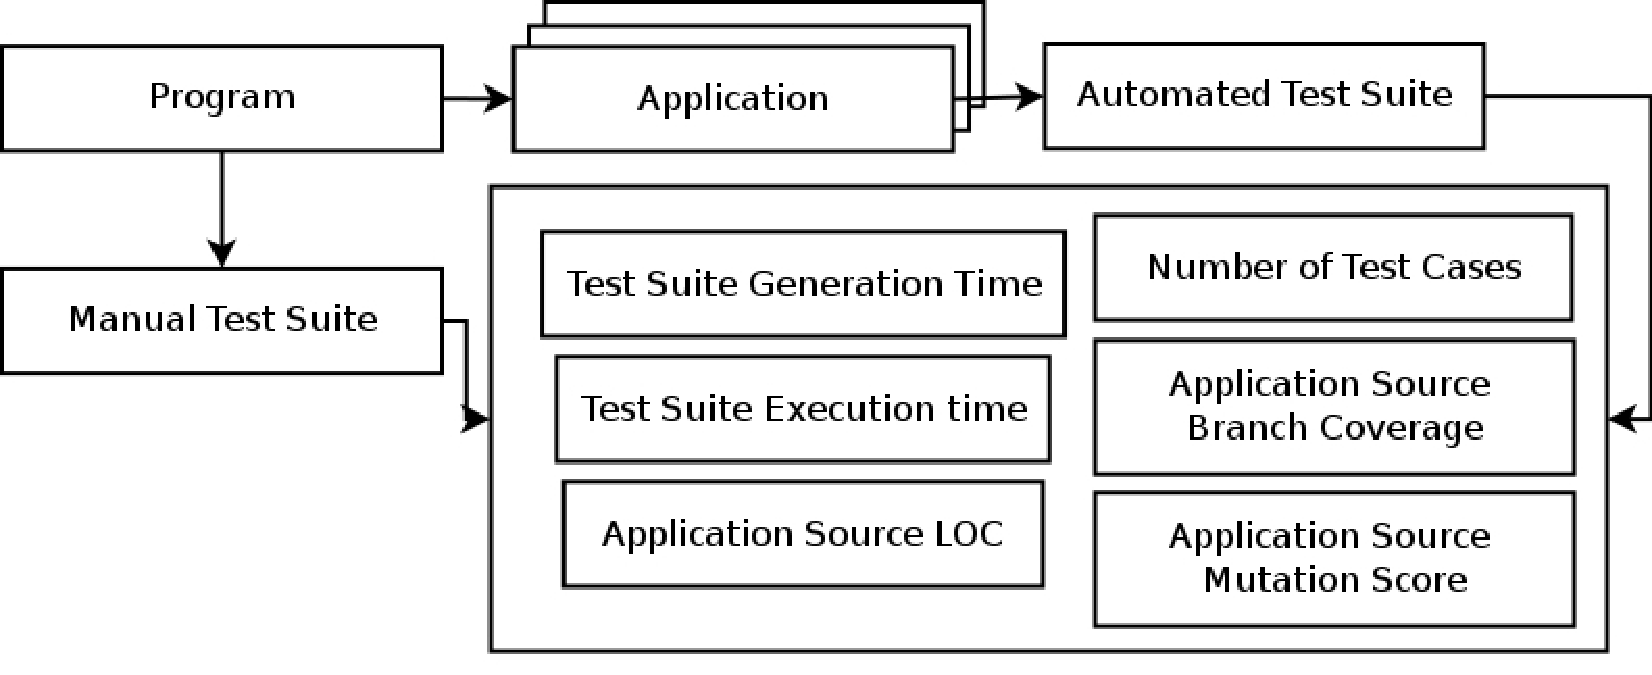
\includegraphics[width=\linewidth]{proccess_diagram.pdf}
    \caption{Evaluation Process}
  \label{fig:process_diagram}
\end{figure}

\section{Empirical Evaluation}
\label{sec:evaluation}
Given the many different techniques for generating test suites, the primary goal of this paper's empirical study is to compare the quality and complexity of the resulting test suites.  We implemented the empirical evaluation approach as shown in Figure~\ref{fig:process_diagram}.  As can be seen in the figure, existing programs are fed into automatic test suite generators to create executable test suites.  These test suites are then compared to the programs' associated, manually written test suites based on 6 different metrics.   

The goals of the experiments are as follows:
\squishlist
\item Do automated or manual test suites create enough quality tests for more complex applications?
\item What is the difference in quality between automated test suite generators and manually written test suites?
\item Does the size of an application  effect the branch coverage and mutation scores of automated and manually generated test suites?
\item Are branch coverage and mutation scores always the best indicators that a test suite reduces cost and effort?
\squishend


\subsection{Experiment Design and Metrics}
All experiments were performed on GNU/Linux workstations with kernel 3.2.0-44, a 2 GHz Intel Corporation Xeon E5/Core i7 processor and  15.6 GB of main memory. 

\noindent \textbf{Case Study Applications:}  

Ten programs were identified from the SF110 code suite~\cite{fraser:2012}.  The case study applications were selected due to their size, the existence of associated manually developed JUnit test cases, and their use in tuning \textsc{EvoSuite} parameters for mutation and test generation, one of our test suite generation tools.  Table~\ref{tbl:program_table} provides a list of the selected SF110 programs with their respective lines of code (LOC) and average cyclomatic complexity per method.  LOC and cyclomatic complexity were measured using JavaNCSS~\cite{leejavancss}.  

%Can cut from this paragraph
Netweaver is the largest program under consideration with nearly 18K lines of code.  Netweaver has an average Cyclomatic Complexity ($CC$) of 2.82 across all methods, which implies that for a specific method $M$, 1) $CC_M$ is an upper bound for the number of test cases that are necessary to achieve a complete branch coverage within the method $M$, and 2) $CC_M$ is a lower bound for the number of paths through the control flow graph. Assuming each test case takes one path, the number of cases needed to achieve path coverage is equal to the number of paths that can actually be taken, ignoring infeasible paths.  The smallest program, Jni-inchi has around 800 lines of code with an average cyclomatic complexity of 2.05.  

\begin{table}[!t]
\caption{Benchmark Programs and their Properties}
\label{tbl:program_table}
\resizebox{\columnwidth}{!}{%
\begin{tabular}{|l|c|c|}
\hline
\textbf{Program} & \textbf{LOC} &\textbf{Cyclomatic Complexity} \\ \hline
Netweaver                              & 17953                              & 2.82                                                \\ \hline
Inspirento                             & 1769                               & 1.76                                                \\ \hline
Jsecurity                              & 9470                               & 2.05                                                \\ \hline
Saxpath                                & 1441                               & 2.10                                                \\ \hline
Jni-inchi                              & 783                                & 2.05                                                \\ \hline
Xisemele                               & 1399                               & 1.29                                                \\ \hline
Diebierse                              & 1539                               & 1.74                                                \\ \hline
Lagoon                                 & 6060                               & 3.52                                                \\ \hline
Lavalamp                               & 1039                               & 1.50                                                \\ \hline
Jnfe                                   & 1294                               & 1.38                                                \\ \hline
\end{tabular}
}
\end{table}

After the case study applications were identified and analyzed, automated test tools \textsc{EvoSuite} and Codepro were used to generate test suites~\cite{CodePro1, fraser:2011:eat:2025113.2025179}. As \textsc{EvoSuite} is non-deterministic and learning-based, ten sets of tests were generated for evaluation, and the standard deviation is given across the ten test generations for all \textsc{EvoSuite} related results.  

\noindent \textbf{Evaluation Metrics:}

The manually written test suites and automatically generated test suites are compared based upon the time to generate test suites, the number of test cases generated, the time to execute generated tests, lines of code in the benchmark application, complexity of the benchmark application, branch coverage of generated suites, and the mutation score of generated suites. To perform these evaluations, three tools are used.

All tests are written or generated in JUnit form.  The time to generate test cases, number of test cases generated, and the time to execute the test suite are measured using the JUnit tool.  We also measure the non-commented LOC from the source code of the benchmark applications through JavaNCSS~\cite{leejavancss}.  

Following the automatic generation of test cases, Jacoco~\cite{jacoco} is used to calculate branch coverage of the tests.  Jacoco calculates branch coverage by instrumenting all branches at the byte code level through ASM, an all purpose Java bytecode manipulation and analysis framework. We also use MAJOR~\cite{just2011} to calculate fault-based mutation scores given the case study and associated tests. MAJOR is a Java compiler-integrated mutator that serves as a mutation analysis back-end for JUnit tests.  It provides a domain specific language to configure the mutation process, although we used its default values for our experiments.

\subsection{Experiments and Results}
Experiments were run to compare how test suites are generated using automated tools, the differences between the resulting test suites in terms of size and complexity, and the over all quality of the generated test suites.  

\subsubsection{Generating Test Suites }
%Time to generate
\begin{figure*}[!t]
\centering
  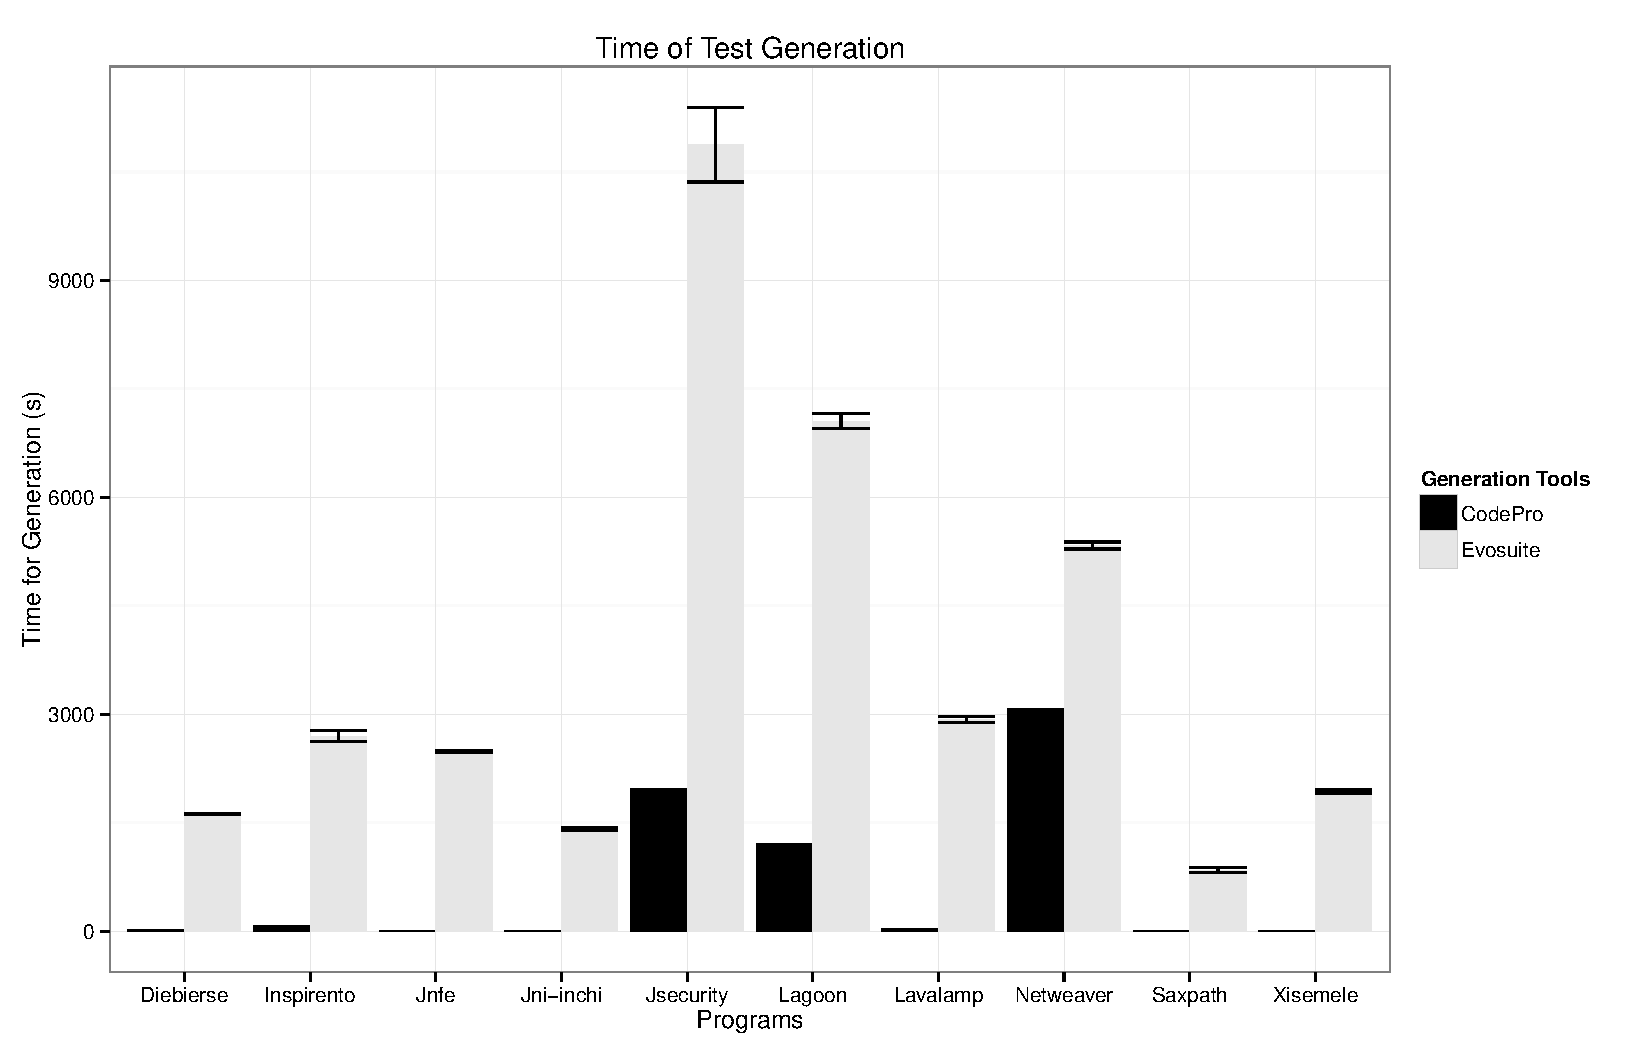
\includegraphics[width=\linewidth, height=11cm]{RGraphs/TimeOfGeneration.pdf}
    \caption{Time to Generate Test Suites.}
  \label{fig:TimeGen}
\end{figure*}
In the first set of experiments, we tracked the time required to generate the test suites, the number of test cases generated, and the execution time of the resulting test suite.  Figure~\ref{fig:TimeGen} displays the time required to generate each test suite using the two automatic test case generation tools, CodePro and \textsc{EvoSuite}.  In the case of Netweaver, CodePro completed test suite generation in approximately 51 minutes whereas \textsc{EvoSuite} required 89 minutes.  This was a small difference of 1.7\% compared to Xisemele, for which CodePro generated a test suite in just 13 seconds compared to 32 minutes from \textsc{EvoSuite}.  The time needed by \textsc{EvoSuite} was 148\% greater in this case.  On average, \textsc{EvoSuite} took 78\% more time in test generation compared to CodePro.

%# of tests
Next, the number of test cases generated per method was analyzed.  Figure~\ref{fig:NumTests} shows the number of tests generated.  For the ten case study applications, CodePro produced an average of  5\% more test cases than \textsc{EvoSuite} and 16.4 \% more than were written manually.  \textsc{EvoSuite} produced, on average, 4\% than were created manually. 

\begin{figure*}[!t]
\centering
  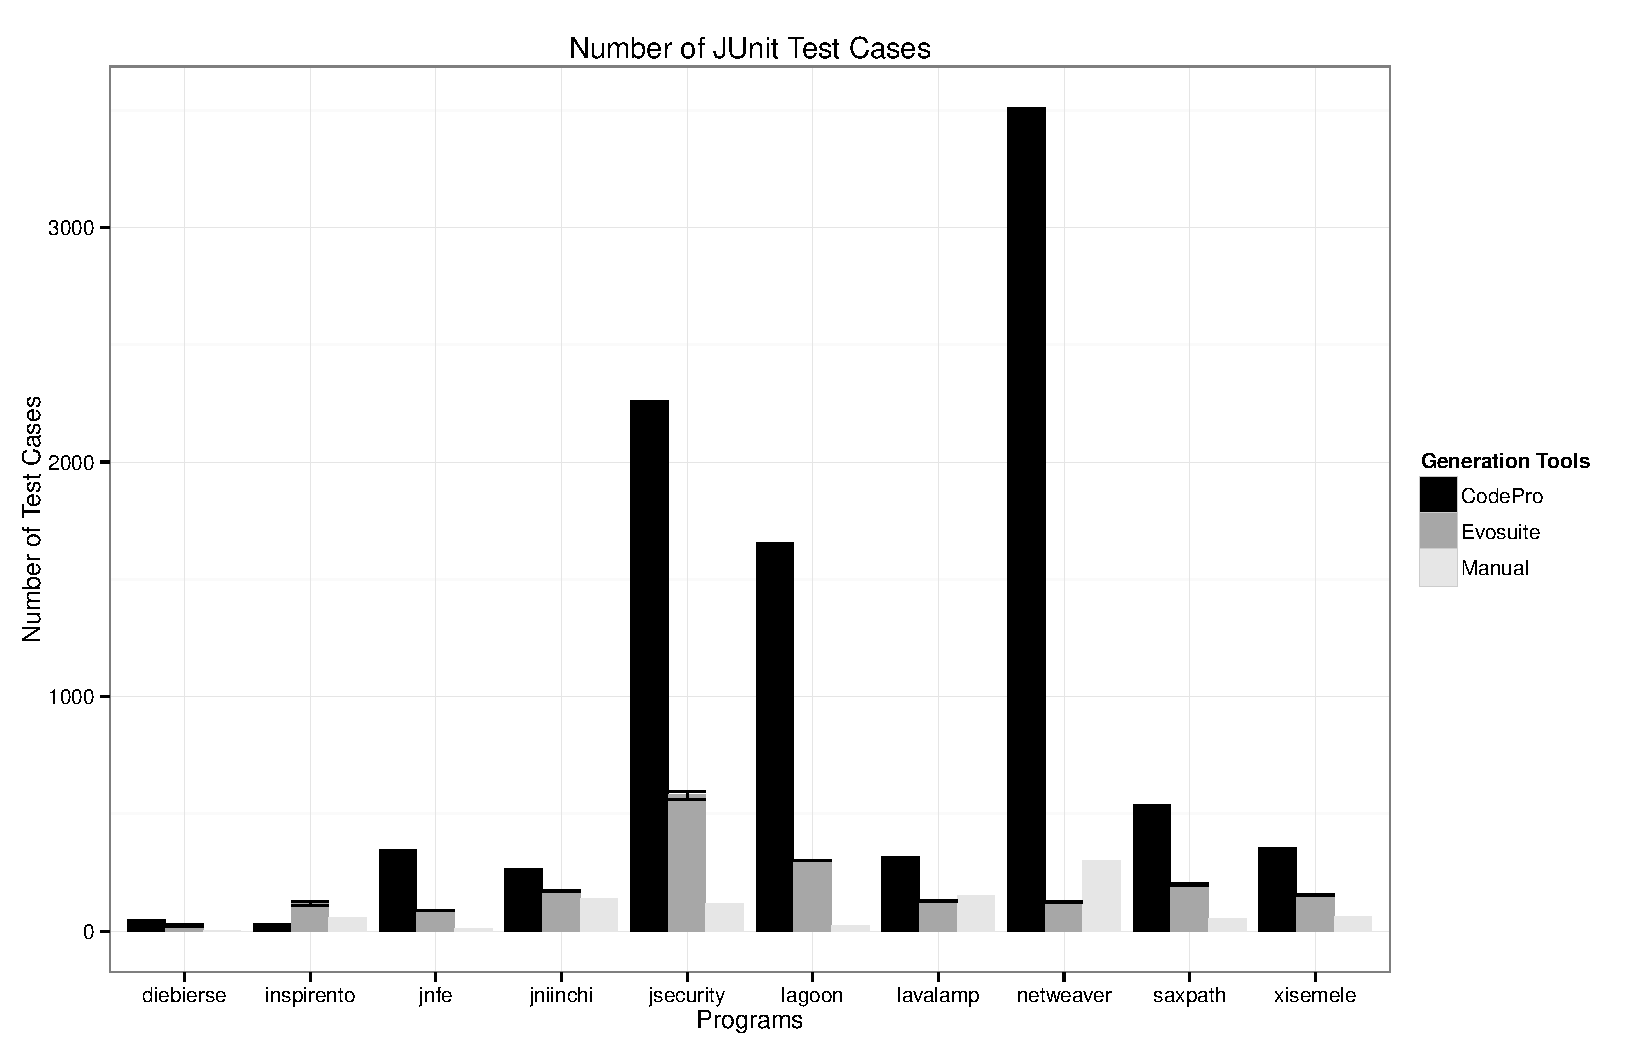
\includegraphics[width=\linewidth, height=11cm]{RGraphs/TestCasesGenerated.pdf}
    \caption{Number of Test Cases per Test Suite.}
  \label{fig:NumTests}
\end{figure*}

%Execution time
The time to execute the generated test suites was also evaluated. Figure~\ref{fig:TestExecTime} reveals that the execution time between manual, \textsc{EvoSuite}, and CodePro test suites, the execution times low ranging between 2.1 to 25.5 seconds to execute. In comparison to Figure~\ref{fig:NumTests}, the netweaver test suite contains the the most test cases. However, the netweaver CodePro test suite does not take the longest to execute, rather, the second largest test suite for jsecurity by \textsc{EvoSuite} does. This may be the result of skeleton-like test cases that CodePro produces. CodePro's skeleton-like test cases provide comments for developers to find where to write test cases, forming a hybrid approach to the automated and manual world of testing.\footnote{ For more information on the composition of these test cases, please reference our material at this web page: http://cs.uccs.edu/~kjustice/QSIC2014/} 

%Time of Execution
\begin{figure*}[!t]
\centering
  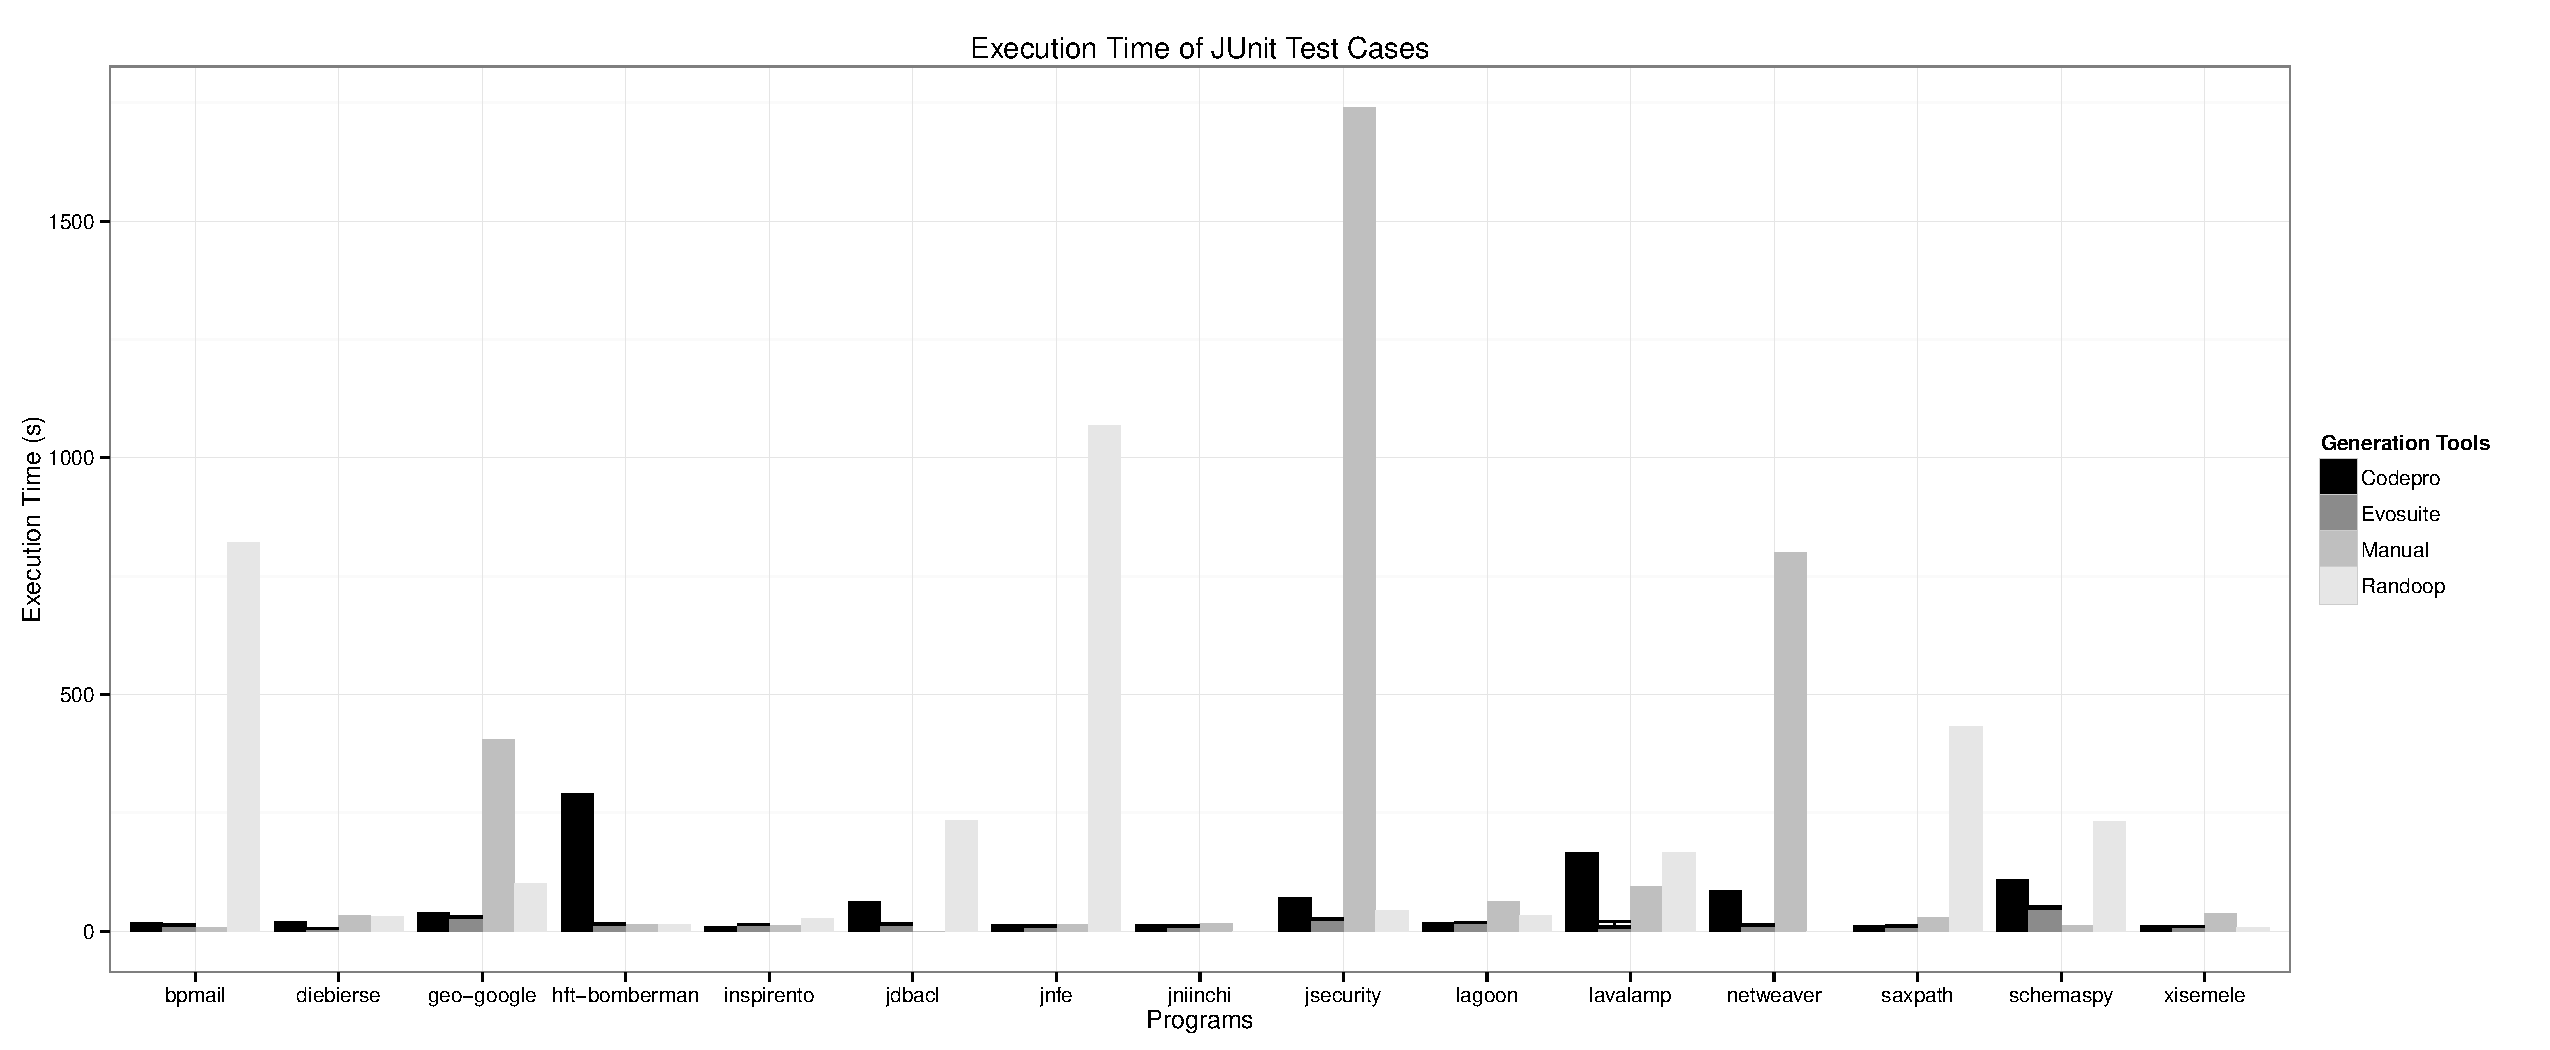
\includegraphics[width=\linewidth, height=11cm]{RGraphs/TestExecutionTime.pdf}
    \caption{Execution Time of all Test Suites.}
  \label{fig:TestExecTime}
\end{figure*}

\subsubsection{Comparing Generated Tests to Case Studies}
%Number of Tests Versus LOC%
%CodPro and and Evosuite retain high $R^2$ values averaging at PERCENT . As the lines of code increases, the number of generated test cases increases. CodePro had by far the most generated test cases and lines of code, averaging over PERCENT more test cases than either Evosuite or the manually written test suites. Evosuite averaged PERCENT more test cases than manual tests. Manual test suites contained the least amount of lines of code and written tests. The overall trend between the LOC and number of test cases for manual were positive, but did not correlate as strongly as the automated test suites did.

%Time to Generate vs Complexity%
%CodePro takes much less time than Evosuite to generate the test suite. Evosuite test generation took PERCENT amount of time longer. Both graphs indicated that more complex applications require longer times to generate test suite. 


%LOC
The LOC for the generated test suites and the application source code were also compared. Figure~\ref{fig:LOC} shows that CodePro generates more LOC than either manual or \textsc{EvoSuite} test suites. As shown in Figure ~\ref{fig:NumTests}, CodePro generated the most tests out of the automated test generators. In a comparison between the two graphs, the a close correlation can be seen between the LOC and the number of tests. For example, netweaver contains 17953 LOC, and CodePro produces 3513 test cases for the application. Likewise, the other applications and their tests suites share this same trend. As the size of the application increases, the number of tests will increase as well. In proportion to the original lines of code, the number of test cases are greatest with CodePro, then \textsc{EvoSuite}, and then manual. 
 
%Branch Cov
%Mutation Score



%LOC (source)
\begin{figure*}[!t]
\centering
  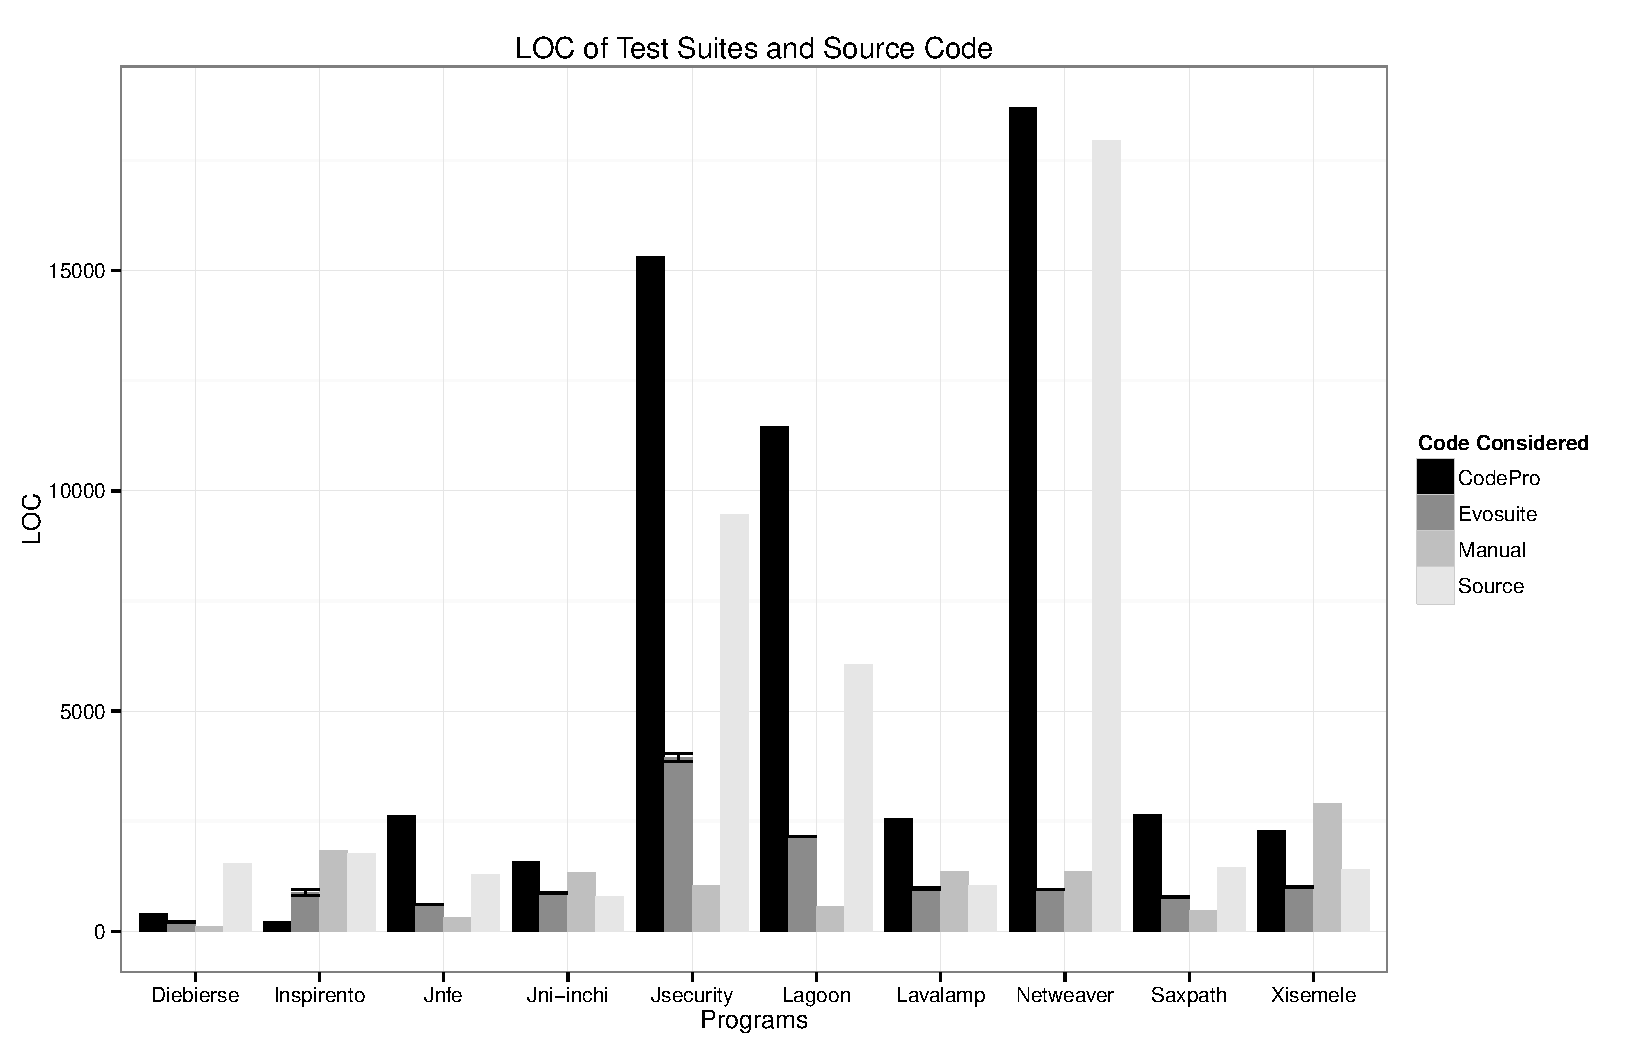
\includegraphics[width=\linewidth, height=11cm]{RGraphs/LOC.pdf}
    \caption{Non-commented lines of code for automatically generated tests and manual tests compared to case study source code. }
  \label{fig:LOC}
\end{figure*}
%Complexity (source)-- do we really compare about complexity of tests versus complexity of source? Leaving out.


\subsubsection{Quality: Manual versus Generated}
In this study, both branch coverage and mutation scores were measured for each of the generation test suites. The branch coverage for manually test suites varied greatly, but was the only method  able to attain a score over 70\% with Lavalamp and Xisemele. Both applications contained the least number of test cases with manual as evidenced by  Figure~\ref{fig:NumTests}. Overall CodePro had higher branch coverage scores than \textsc{EvoSuite} or manual. This could indicate a direct relationship between the number of tests and the branch coverage. 

%Number of Tests vs Branch Coverage%
The relationship between the number of tests and the branch coverage for each test generated suite was furthermore examined. In comparing Figure~\ref{fig:NumTests} and the branch coverage, manual test suites increased in branch coverage as the number of test cases increased. When evaluating \textsc{EvoSuite}, the trend line has a low  $R^2$ value at 0.184, but begins in a similar trend to manual and CodePro, and actually drops in branch coverage for the two larger test suites. The branch coverage in comparison with the number of tests indicates that CodePro branch coverage drops as the number of generated test cases increases. Larger applications may require more tests to be written to increase the branch coverage. 

%\begin{figure}[!t]
%\centering
 % 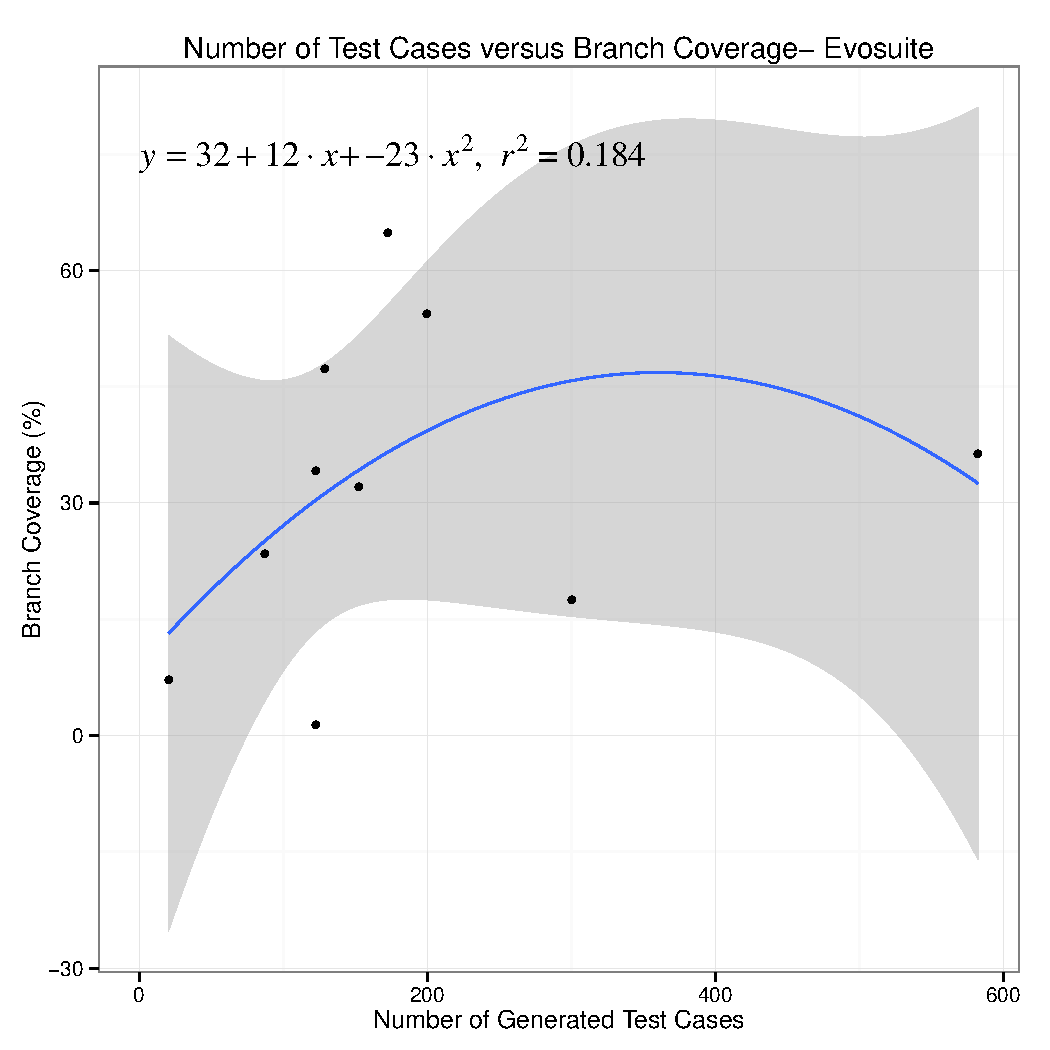
\includegraphics[width=\linewidth]{RGraphs/Evosuite_TestsVersusBranchCov_poly.pdf}
 %   \caption{Number of tests compared to the branch coverage of Evosuite.}
 % \label{fig:NumTestsvsBranchCov}
%\end{figure}





%LOC vs Branch Coverage%	
The research evaluated the relationship between LOC and Branch coverage for each of the generated test suites.  \textsc{EvoSuite}, CodePro, and manual test suites in Figure a similar trend in the decrease of Branch Coverage as the LOC of the application code increased. Only CodePro displays a larger increase in branch coverage by at least 27\%  more for the largest program netweaver in comparison with  \textsc{EvoSuite} and manual. Despite generating more tests in proportion to the application source code size,  CodePro did not meet the quality of the tests generated by \textsc{EvoSuite} and the manual written test suites.

\begin{figure}[!htbp]
\centering
  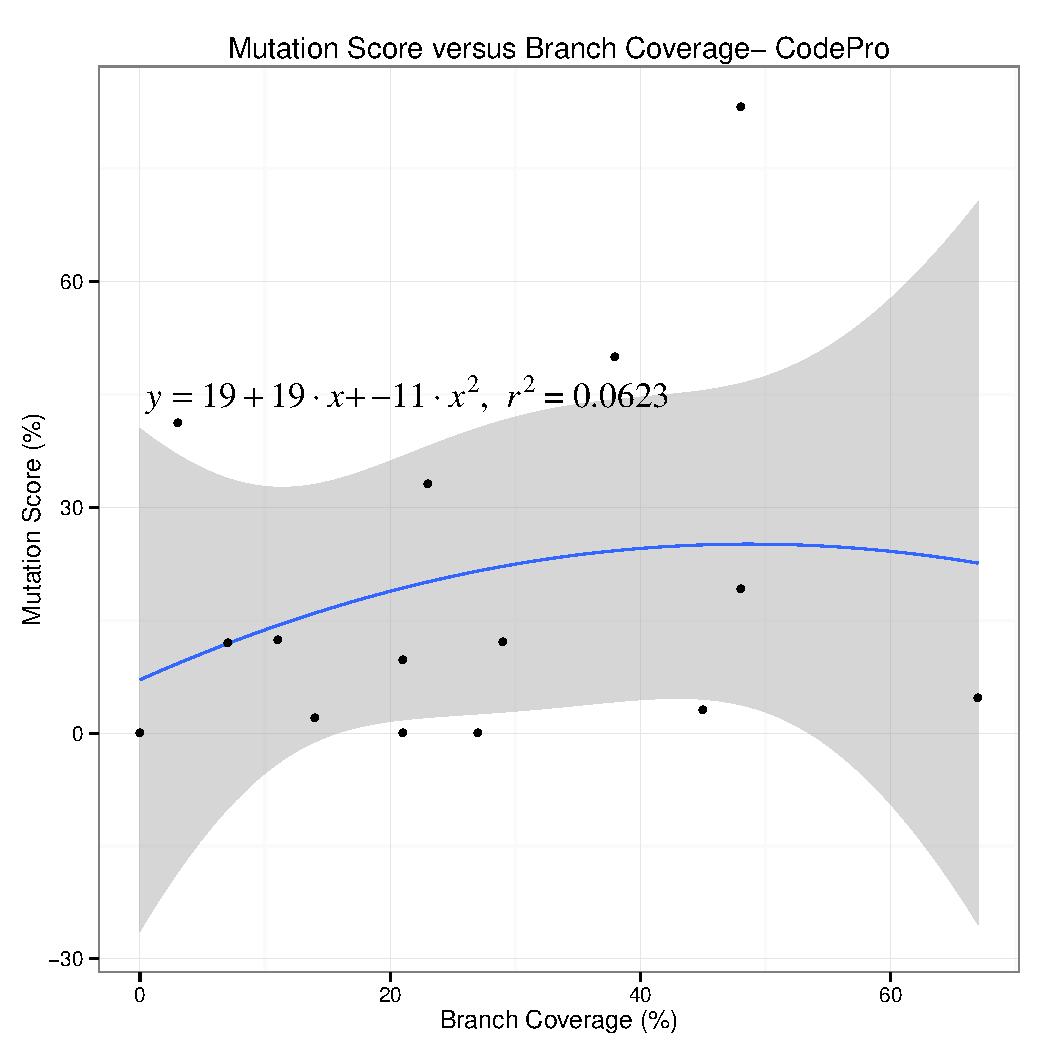
\includegraphics[width=\linewidth]{RGraphs/CodePro_BranchCov_versus_Mutation_poly.pdf}
    \caption{Mutation Score compared to Branch Coverage for test suites generated by CodePro.}
  \label{fig:CP_branch_mutation}
\end{figure}
%Mutation score%
For the mutation score, \textsc{EvoSuite} attained the highest scores for five of ten applications. However, dieberse scores ranged dramatically between 18\% and 40\%.CodePro resulted in the worst mutation scores, acquiring a  0\% mutation score for lagoon, saxpath, and xisemele. None of these three programs showed any close correlation to the 0\% mutation score. \textsc{EvoSuite} however was able to generate test suites averaging between 33.7\% and 77.1\% for these applications. Manual tests remained between 18.3\% and 56.5\%  between the applications, while CodePro mutation scores ranged between 0\% and 41.3\%. 


%Branch Coverage vs Mutation%
This research compared the branch coverage to the mutation scores of the generated test suites. In Figures ~\ref{fig:manual_branch_mutation} and ~\ref{fig:Evo_branch_mutation}, the mutation score increased as the branch coverage increased as the mutation score increased.  Figure ~\ref{fig:CP_branch_mutation} displays a much lower $R^2$ value at 0.137, but the data indicates overall that the mutation score neither increases nor decreases with higher branch coverage. This can be explained because the mutation scores were all much lower than manual and  \textsc{EvoSuite} scores. With exception to the out-lier of a 40\% mutation score, the trend would otherwise indicate that the mutation score increases as the branch coverage increases.


%Complexity vs Mutation%
%We further examined the relationship between the Cyclomatic Complexity of the application source code and the mutation score of the generated test suite. For manual test suites, Figure MANUAL indicates that applications with a higher complexity received lower mutation scores. Figure EVOSUITE shows that the two most complex programs that manual test suites received the lowest mutation scores for received just about the same scores as less complex applications with Evosuite. Less complex applications received overall higher mutation scores with Evosuite. Figure CODEPRO reveals that the most and least complex programs both received mutation scores of 0. Regardless of complexity, all of the mutation scores are low for CodePro.

\begin{figure}[!htbp]
\centering
  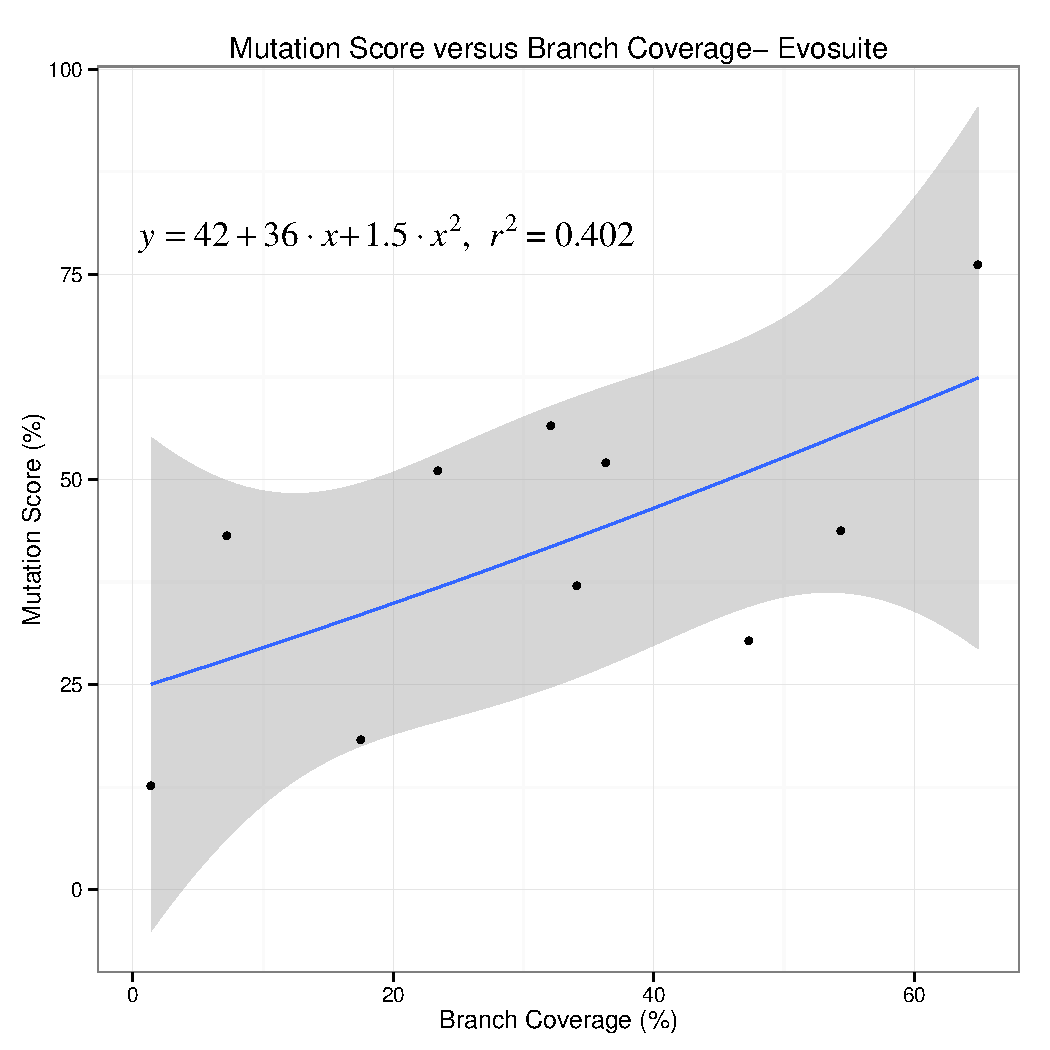
\includegraphics[width=\linewidth]{RGraphs/Evosuite_BranchCov_versus_Mutation_poly.pdf}
    \caption{Mutation Score compared to Branch Coverage for test suites generated by Evosuite.}
  \label{fig:Evo_branch_mutation}
\end{figure}

\begin{figure}[!htbp]
\centering
  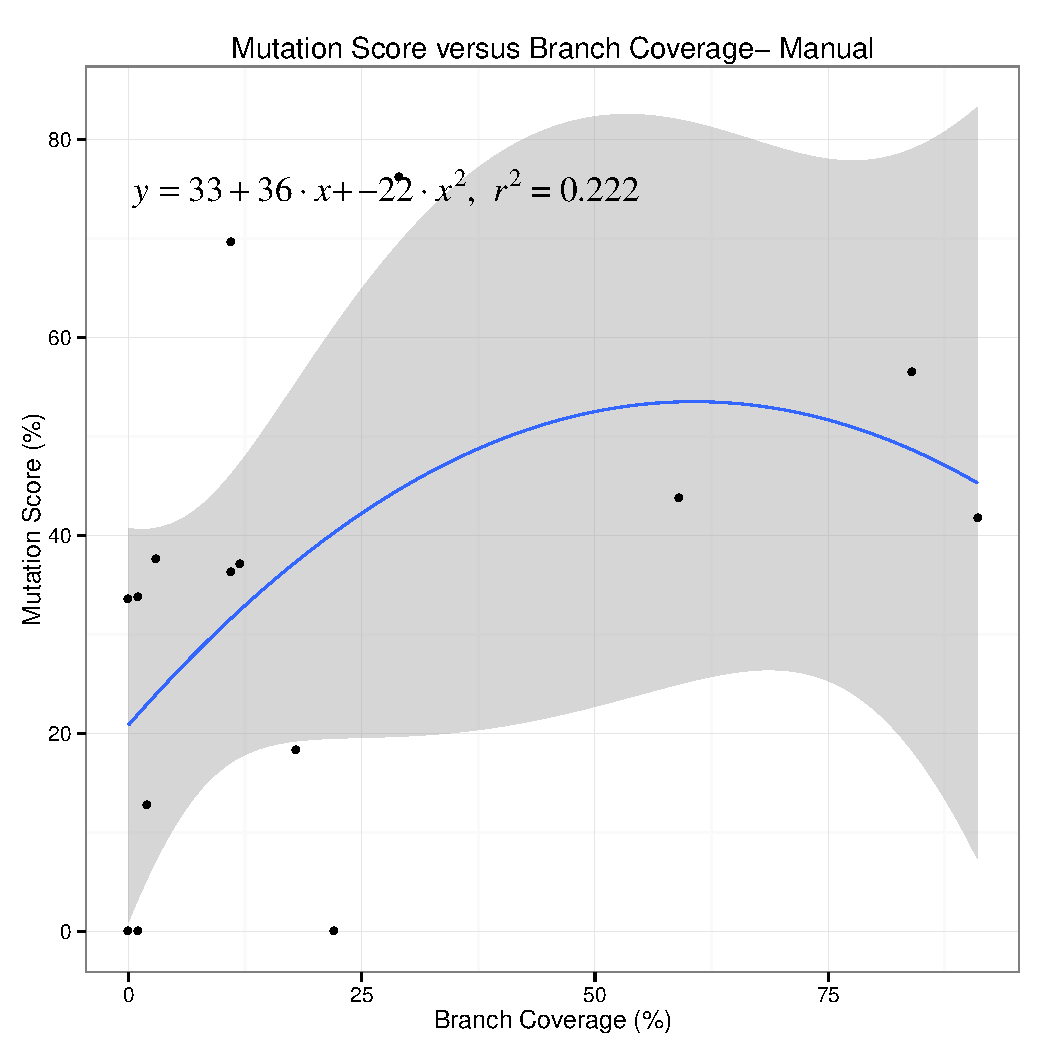
\includegraphics[width=\linewidth]{RGraphs/Manual_BranchCov_versus_Mutation_poly.pdf}
    \caption{Mutation Score compared to Branch Coverage for test suites created manually.}
  \label{fig:manual_branch_mutation}
\end{figure}

%More info%
For further results from our evaluations related to LOC of the generated test suites, cyclomatic complexity of the test suites, and cyclomatic complexity of the application source code, please reference our web page: http://cs.uccs.edu/~kjustice/QSIC2014/. 


\subsection{Threats to Validity}
\noindent \textbf{Internal Validity}
Threats to internal validity include the 

Measurements in quality of software tests is a subjective measurement. Although mutation score is one way to measure the quality of a test suite, ignoring the human elements of tests are nigh impossible. Developers may need to view tests in order to diagnose faults in the code, and if a developer cannot understand the test they are reading, then the cost of time and effort could be increased on the human part.

The statistical analysis also may be a threat to validity, as the inconsistency in how both \textsc{EvoSuite} and manually written tests are created. Also, CodePro generated some test suites with a mutation score of 0, which could mislead one to believing that CodePro has no use for creating quality tests. For this reason we removed these results to give a better impression of the trend CodePro test suites.


%\noindent \textbf{External Validity}

%\noindent \textbf{Construct Validity}


\section{Discussion}
\label{sec:discussion}
In comparison with LOC and the number of Test Cases, it would seem that the higher proportion of Test Cases to the original application code does not necessarily imply that either or both the mutation score and branch coverage will be high.  Especially in the case of CodePro, in which many tests are produced in a skeleton-like fashion, the mutation scores and branch coverage are much lower than  \textsc{EvoSuite} and manual tests. However, as indicated earlier, the skeleton approach to generation gives developers a template to easily modify and implement. With the quick generation that covers a large scope of the application, developers are not required to spend time or effort looking for where the test should be, but rather enhancing them later. This feature could be more desirable to those who would like the higher coverage from an automated test suite like  \textsc{EvoSuite}, but have the flexibility to write the quality of tests relieved from manually generated tests.

From a pure comparison of quality between \textsc{EvoSuite}, CodePro, and manually written test suites, manual test suites have the potential for attaining the highest coverage and mutation scores. Potential can only be measured by the individual writer of the tests, and could be one of the reasons the data relating to the manual test suites are less consistent than that of \textsc{EvoSuite} and CodePro. \textsc{EvoSuite} almost retains the same quality as Manual tests, achieving an average of only one percent less in total for mutation score of \textsc{EvoSuite} at 39.8\%  and manual with 40.3\%. \textsc{EvoSuite} would reduce the time and cost of implementing the tests in comparison to manual tests. Also \textsc{EvoSuite} can maintain the relative quality as manual tests, but provide little modifiability of the tests, as the genetic algorithm changes the test suite every time.

%!TEX root=qsic2014.tex
% mainfile: qsic2014.tex

\section{Related Work} \label{sec:related_work}

Since this paper focuses on empirically comparing manually implemented and automatically generated test suites, it is most directly related to Bacchelli et al.'s evaluation of the effectiveness of manual and automated test data generation~\cite{bacchelli2008}. However, there are several distinctions between our paper and this prior work. While the experiments in this paper focus on test suites for ten case study applications, Bacchelli et al.\ only consider select classes that implement data structures like {\tt LRUHashtable}. In contrast to the use of manual tests that were implemented by real-world open-source software developers, the manually-coded test cases in Bacchelli et al.'s were created by the authors themselves.  Moreover, Bacchelli et al.\ use Randoop~\cite{pacheco2007feedback} and JCrasher~\cite{csallner2004}, instead of picking \textsc{EvoSuite}, the current state-of-the-art test data generation tool~\cite{fraser2013a}. Finally, it is important to note that even though Bacchelli et al.\ report coverage and mutation scores, they neither investigate the correlation between coverage and mutation nor perform a comprehensive statistical analysis of the results. In addition, it is possible to make similar comparisons between our paper and the experimental work of Assylbekov et al.~\cite{assylbekov2013}.

The design of the our paper's experiments is informed, in part, by the experimental design and results presented by Inozemtseva and Holmes~\cite{inozemtseva2014}. Like our paper, this prior work also uses real-world programs to empirically investigate the relationship between code coverage and mutation score. However, the primary intent of our work is different than that of Inozemtseva and Holmes: while they investigate the effectiveness correlation for the test suites that come with programs, we consider both manually and automatically generated tests. Moreover, it is important to note that while their paper uses PIT~\cite{pit2014} for fault seeding, our experiments use MAJOR---the only mutation testing tool whose mutants are currently known to be statistically similar to real-world faults~\cite{just2014}.

Our paper's experiments are also partially influenced by the design and results reported on by Gopinath et al.~\cite{gopinath2014}.  This paper is similar to ours because it also investigates the correlation between a test suite's coverage and mutation score.  In addition, Gopinath et al.\ use both manually and automatically generated test suites for more programs than we do; yet, since our experimentation framework is easy to apply to new programs and our presented results demonstrate promise, we will scale our study to Gopinath et al.'s level in future work. Moreover, even though \textsc{EvoSuite} automatically generates better test suites than Randoop~\cite{fraser2013a}---thus motivating its use in our experiments---Gopinath et al.\ use Randoop to create test suites.  In addition, while Gopinath et al.\ employ PIT to seed faults into their case study applications, we decided to use MAJOR since recent results indicate that this tool's faults are a valid substitute for real faults~\cite{just2014}. 

Ultimately, the results from Inozemtseva and Holmes \cite{inozemtseva2014} and Gopinath et al.~\cite{gopinath2014}, in conjunction with those in this paper, present a complementary understanding of the effectiveness of automatically and manually generated test suites. It is also important to remark that, while Just et al.~\cite{just2014} are the first to establish a statistical correlation between a test suite's mutation score and its effectiveness at detecting real-world faults, the purpose of that work is not to develop a full-featured understanding of the quality characteristics of automatically and manually generated test suites---the aim of our paper.

% There are few studies comparing the quality of manual and automated test suites. In one study researchers found that
% using automated test generation tools did not improve the ability to test the software~\cite{fraser2013c}. However, the
% study does not measure the quality of manual and automated generated test suites directly.  Furthermore, only Evosuite
% is used to evaluate the mutations and generate the tests.  This paper expands upon the question of the usefulness of
% automated generated test suites, and if certain systems in generating test suites work better than others.

It is important to note that all of the aforementioned related work focuses of the empirical and technical aspects of test suite effectiveness that are not related to human-centric issues.  In part, our paper was motivated to investigate the complexity and understandability of automatically and manually generated test suites by Fraser et al.'s empirical results revealing that automatically generated tests do not always help software testers find more defects in a program~\cite{fraser2013c}.  While Fraser et al.\ also consider coverage and mutation scores for automatically and manually generated test suites, they only use one automated test suite generator, \textsc{EvoSuite}, while we additionally consider tests created with a deterministic tool called CodePro.

In contrast to our focus on manually and automatically generated test suites for real-world open-source applications, other related work has considered coverage and mutation scores for test suites written by students. For instance, Aaltonen et al.\ observe that automated grading programs may reward students for high-coverage test suites that actually have poor defect-revealing potential~\cite{aaltonen:2010:mav:1869542.1869567}, concluding that a combination of coverage and mutation scores may be the best way to give students accurate feedback on the quality of their test cases.  In addition, Shams and Edwards experimentally observe that mutation scores are lower than coverage values for student-implemented test suites~\cite{shams2013}---a result that corresponds to what we found for open-source programs.

There are a wide variety of past empirical studies that compare different coverage criteria; due to space constraints we
briefly review the most relevant work in this paper. For instance, Frankl et al.\ experimentally compare the all-uses dataflow
criterion to mutation adequacy, finding that, although mutation testing is more expensive that dataflow testing, neither
approach was obviously better than the other~\cite{frankl1997}. As an additional example, Gligoric et al.\ also use
mutation testing to empirically compare the effectiveness of non-adequate test suites that aim to fulfill different
adequacy criteria, revealing that branch coverage and intra-procedural acyclic path coverage are the best
\cite{gligoric2013}.

% Another paper compares measuring quality between faults detection and mutation scores~\cite{just2014}. The research
% statistically proves that mutation score can be used as a test of quality of test suites in place of fault detections.
% The paper uses automated test suites to validate this research, and unlike this paper's research, the author's do not
% compare mutation score, branch coverage, and cyclomatic complexity as joint measurements of quality. 

There is research comparing multiple mutation analysis tools~\cite{ComparingAutomatedMutationTools:2013}. This paper differs from this research in specifically comparing mutation analysis tools for Java. MAJOR was recommended as one one of the premier tools, and was thus used for the evaluation.

\section{Conclusions and Future Work}
\label{sec:conclusion}
%----------------------------------------------------------------------------------------------------------------------------------------------------------------------------------------------------------------------------------
Developers have struggled to find a standard of measuring the quality of tests. Mutation testing and seeding faults has proven as one effective way to identify lower quality tests, and many developers consider high branch coverage a sufficient mark of quality for their test suites. The dilemma becomes a cost trade off between depth and breadth, two measurements that this paper uses to address quality. If mutation analysis results represent the depth of test suites, and branch coverage represents the breadth of test suites, the results of this research identifies trends between the automated tools and developers who write tests. Mutation scores and branch coverage correlate in a positive fashion between the two.

Complexity of the program appeared to also influence the mutation score and time to generate the test suite. In the case of the time needed to generate the test suite, a tool utilizing a genetic algorithm took much longer than a deterministic algorithm to generate test suite. However, the cost of time could be outweighed by the better quality received in the mutation scores. The genetic algorithm sustained a higher mutation score than even the manually written tests when the programs were larger. It may be that automated test tools cover larger programs better than manual tests do.

This paper also addresses new questions. First, what is the purpose of auto generating test suites? CodePro garnered poor scores for both mutation and branch coverage results. Although the quality suffered, the research revealed that the CodePro tests were modifiable. Perhaps some tools could be used assist developers in developing a test suite with a template, placing a focus on modifiable tests rather than a complete test suite to match the quality of manually written tests.

Secondly, what is the future of genetic algorithm based tools such as Evosuite? The tests may not be as modifiable as CodePro's, but the mutation scores in some cases matched and exceeded the mutation scores of manually written tests. If the cost of time and effort given from running Evosuite is less and will generate almost the same results for a large program, perhaps developers ought to consider using a tool like Evosuite.

Finally, the paper identifies the inconsistencies between manually generated tests. There is no way one can say with certainty that the goal of each of the developers for each of the projects was to achieve a high mutation score or high branch coverage. Perhaps developers only care to test one function of the code in depth, or rather they would seek to achieve a high branch coverage. Either way, the intentions of achieving the quality standards outlined in this paper may not be ideal for every developer. 

%GREG\KRISTEN - Will we need something like this?
%In order to reproduce this study and further research in software testing, please reference our material on our web page:

 %http://cs.uccs.edu/~kjustice/QSIC2014/

\section{Acknowledgements}                                                       
We thank Ren\'e Just for his comments on earlier versions of this paper and for his support with the MAJOR system. 
We thank Gregory Kapfhammer for his insight and comments on earlier versions of this 
paper.

\bibliographystyle{IEEEtran}
\bibliography{sample}
%\balancecolumns 

\end{document}
